\begin{chapter}{General algorithm for spawning and propagation}
\label{ch:spawncrossgeneral}

In this chapter we try to develop a generalized algorithm for combined
propagation and spawning of wavepackets. The idea is to extend the algorithm
\ref{al:spawning_propagation_na_simplified} to be applicable to arbitrary
non-adiabatic potentials. There are several interesting open questions and
we can state some hopefully worthwhile goals for further research.

\section{Motivating example}

An example motivating the complicated algorithms developed in this chapter is now
examined in much detail. The potential we analyze has two energy levels $\lambda_0$
and $\lambda_1$ and is given by the following matrix

\begin{equation*}
  V\ofs{x} =
  \left(\begin{smallmatrix}
  \tanh\ofs{\rho + x} \tanh\ofs{x - \rho} & \delta\\
  \delta                                  & - \tanh\ofs{\rho + x} \tanh\ofs{x - \rho}
  \end{smallmatrix}\right)
\end{equation*}

where $\rho \in \mathbb{R}$ and $\delta$ is the gap size again. In the example
we set $\rho=3$. The potential is shown in the background of figure \ref{fig:double_gap}.
This figure shows four snapshots from a simulation. In the first panel we see the
initial configuration where we start with $\Ket{\Psi_0} = \phi_0$ on the upper level
and to the left of both avoided crossings. The wavepacket has a momentum to the
right. When the packet passed the first crossing it will split up into two parts,
one on each energy surface. Already now we could ask why we want to keep both
parts inside the same mathematical wavepacket. After the last chapters a split
and spawn procedure comes into mind immediately. If we now split up the packet
$\Psi_0$ according to $\Psi_0 \rightarrow \Psi_1 + \Psi_2$ we end up with two
packets after the first crossing which are mathematically independent but still
can interact physically. (We also set the characteristic component $\chi$ for both
packets according to $\chi_{\Psi_1} \assign 0$ and $\chi_{\Psi_2} \assign 1$ thus
the packet $\Psi_1$ is the part on the upper level.)

The $\Psi_2$ on the lower level moves faster than the one on the upper level.
And thus the two packets will separate further and further in the
long run. For this reason our decision to split and spawn was right. If the potential
had only a single crossing we could stop now, but this potential has two crossings
and we have to go on with our thought experiment. The packet on the lower level will enter
the region of the second avoided crossing first. We assume the linear part between
the two crossings being sufficiently long such that the packets have separated
enough to enter the second crossing after each other. This is true for the
example shown below. As now $\Psi_2$ passed the second crossing a part of it will
go to the upper level $\lambda_0$ again hence the packet splits once more. If we
follow this split mathematically and change the representation we have to spawn
again and write $\Psi_2 \rightarrow \Psi_3 + \Psi_4$ with $\chi_{\Psi_3} \assign 0$
and $\chi_{\Psi_4} \assign 1$. At that time we already have three active wavepackets,
namely $\{\Psi_1, \Psi_3, \Psi_4\}$ and the first two of these reside on the upper
level.

Some time later the back-most packet $\Psi_1$ on the upper level will finally
enter the second crossing. And you guess it, part of this packet will jump to
the lower level. Once more we should split and formally write $\Psi_1 \rightarrow \Psi_5 + \Psi_6$
where $\chi_{\Psi_5} \assign 0$ and $\chi_{\Psi_6} \assign 1$. (These assignments
are of course arbitrary and solely change the notation.)

\begin{figure}[h!]
  \centering
  \subfloat[][]{
    \label{fig:double_gap_frame1}
    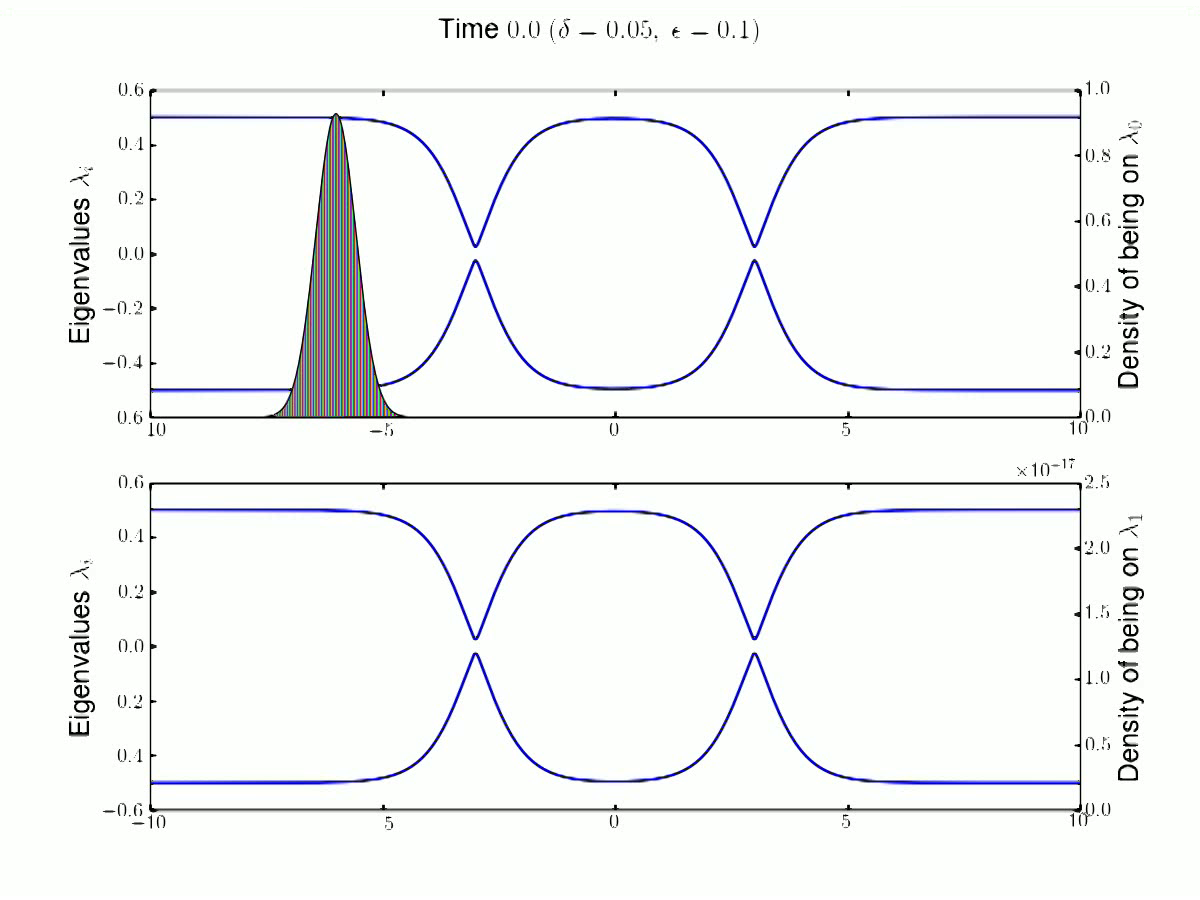
\includegraphics[width=0.5\linewidth]{./figures/double_gap/frame1.png}
  }
  \subfloat[][]{
    \label{fig:double_gap_frame2}
    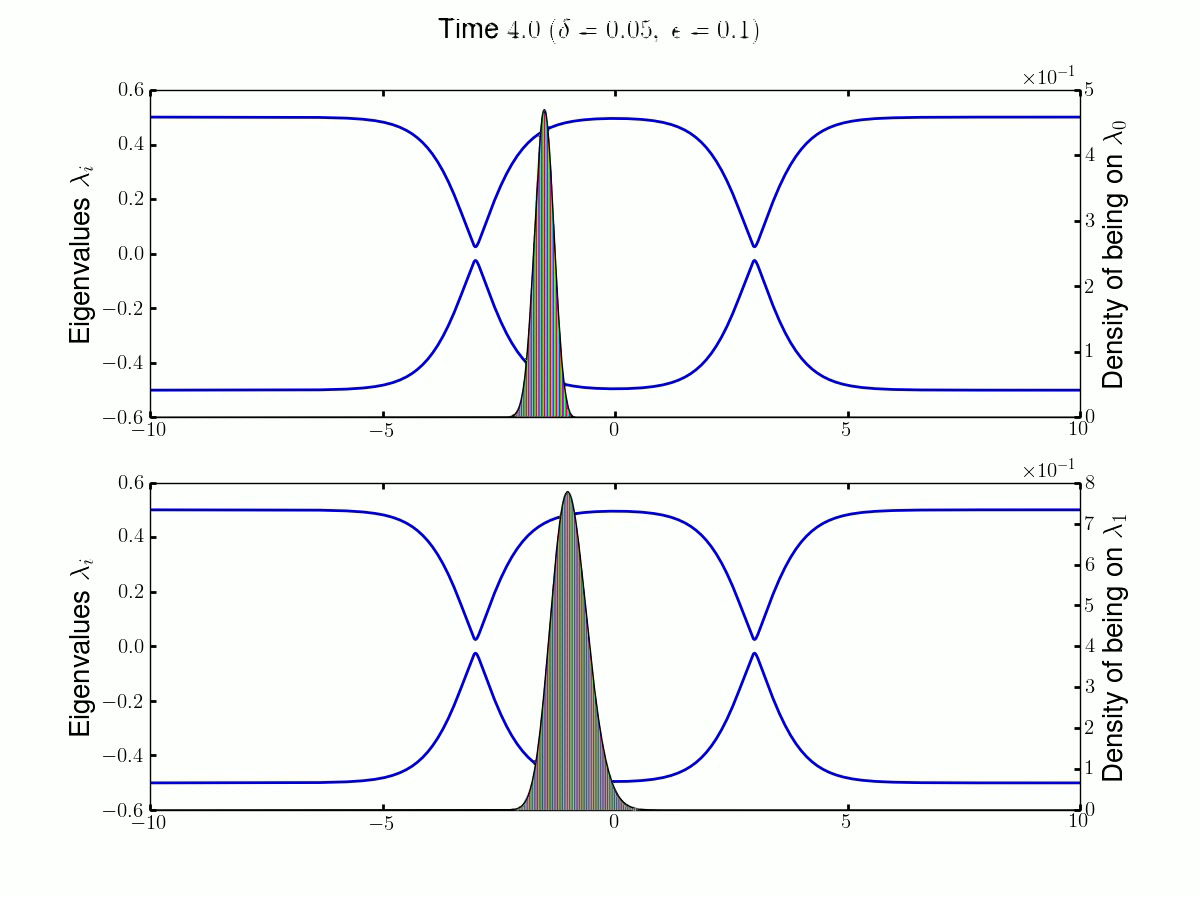
\includegraphics[width=0.5\linewidth]{./figures/double_gap/frame2.png}
  } \\
  \subfloat[][]{
    \label{fig:double_gap_frame3}
    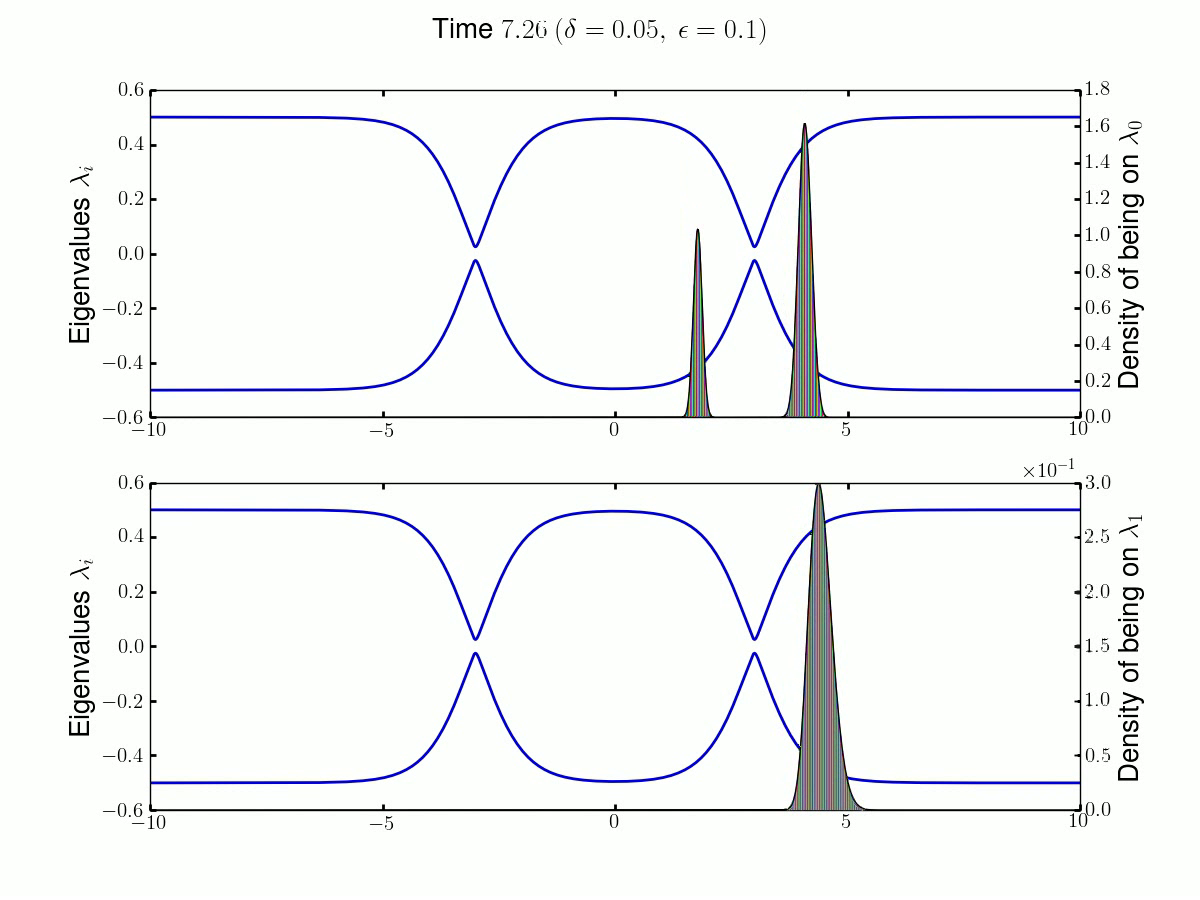
\includegraphics[width=0.5\linewidth]{./figures/double_gap/frame3.png}
  }
  \subfloat[][]{
    \label{fig:double_gap_frame4}
    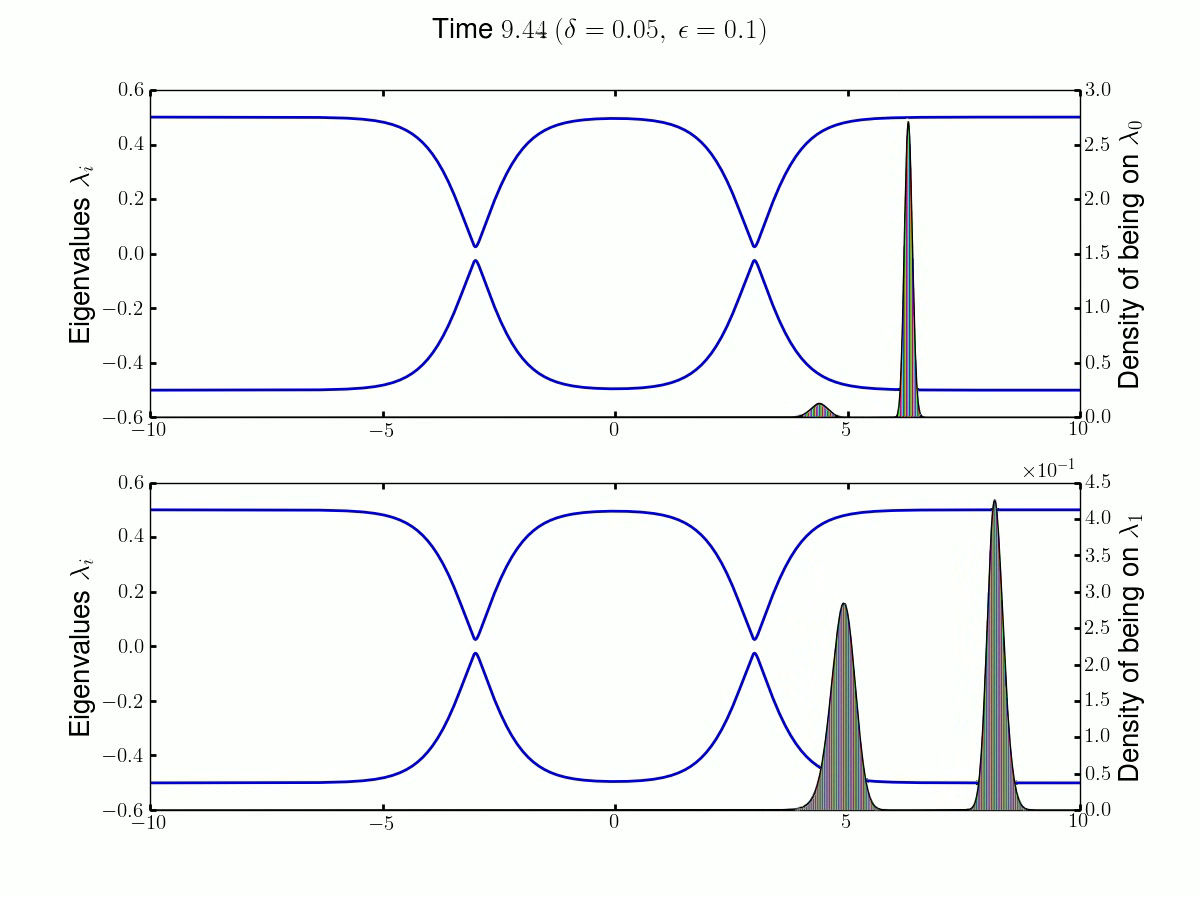
\includegraphics[width=0.5\linewidth]{./figures/double_gap/frame4.png}
  }
  \caption[Motivating example for general spawn propagation algorithm]{
  The potential here has two avoided crossings. We start with a single
  Gaussian wavepacket on the upper level coming from the left. We see
  that at each crossing the packet splits up into two new Gaussian packets.
  This should be motivation enough for a general spawning algorithm.
  Notice the different scales on the y axis for both energy levels!
  }
  \label{fig:double_gap}
\end{figure}

We see that already a relatively simple potential exhibits very complex dynamics.
We start with a single wavepacket $\Psi_0$ which has a Gaussian shape and end up
with \emph{four} wavepackets $\{\Psi_3, \Psi_4, \Psi_5, \Psi_6\}$ at the end of
the day. The final wavefunction after both crossings is then given by $\Psi_f = \Psi_3 + \Psi_4 + \Psi_5 + \Psi_6$.
It should be clear by now that it does not make any sense to keep these four parts
inside the same (mathematical) wavepacket $\Ket{\Psi}$. What would the optimal
choice of the parameter set $\Pi$ be for this packet? Additionally we would need
an exceedingly large basis to represent all parts accurately. (This is by the way
the reason why the above simulation was not possible with the wavepacket based algorithms
from \cite{FGL_semiclassical_dynamics} and \cite{BGH_nonadibatic_algorithms} for
small but interesting gap sizes of $\delta \approx \varepsilon$. The example stems
from a simulation done with Strang splitting of the propagation operator.) Just
for fun we could briefly imagine a potential matrix like the following one

\begin{equation*}
  V\ofs{x} =
  \left(\begin{smallmatrix}
  \prod_i\tanh\ofs{x-\rho_i} & \delta\\
  \delta                     & - \prod_i\tanh\ofs{x-\rho_i}
  \end{smallmatrix}\right)
\end{equation*}

for a whole set $\{\rho_i\}_{i=1}^n$. This potential consists of $n$ avoided
crossings in series. And the initial wavepacket $\Ket{\Psi_0}$ could in the
worst case split up into $2^n$ packets because we can double the number of packets
at each crossing!


\section{Some notations}

For the next section we have to extend our notations around wavepackets with
some smaller additions. The (homogeneous) vector valued wavepacket having $N$
components is given by (copied from \eqref{eq:hawp_def_state_vector})

\begin{align}
  \Ket{\Psi} & \assign \Ket{\left(\Phi_0, \hdots, \Phi_{N-1}\right)} \,.
\end{align}

Now we define the restriction operator which reduces the wavepacket to a single
component $\Phi_j$ by

\begin{align}
  \Ket{\Psi |_j} &
  \assign
  \Ket{\left(0, \hdots, 0, \Phi_j, 0, \hdots, 0\right)} \,.
\end{align}

Thus the wavepacket $\Psi$ gets reduced to the component that is localized on the
energy level $\lambda_j$. In principle this is the same as extracting $\Phi_j$
from $\Psi$ but with this new definition we keep the vector structure of $\Psi$.

The definition of the restriction to the complement works alike. If $j \in [0, N-1]$
then the complement $\bar{j}$ is defined as $\bar{j} \assign [0, N-1] \setminus \{j\}$
and therefore

\begin{align}
  \Ket{\Psi |_{\bar{j}}} &
  \assign
  \Ket{\left(\Phi_0, \hdots, \Phi_{j-1}, 0, \Phi_{j+1}, \hdots, \Phi_{N-1}\right)} \,.
\end{align}

With this operator we can zero out the component $\Phi_j$ of $\Psi$ and remove
the part localized on the energy level $\lambda_j$.


\section{Wavepacket superpositions and interactions}

Presume for this section that our wavefunction $\varphi$ is represented not by a
single homogeneous or inhomogeneous wavepacket $\Psi$ but instead by a linear combination
thereof. Formally we write

\begin{equation}
  \Ket{\varphi} = \Ket{\Psi_0} + \Ket{\Psi_1} + \ldots + \Ket{\Psi_{J-1}} = \sum_{j=0}^{J-1} \Ket{\Psi_j} \rassign \Ket{\Upsilon}
\end{equation}

and use this as primary definition for $\Ket{\Upsilon}$ which we call a \emph{superposition}.
In the motivating example we have as initial condition $\Ket{\Upsilon} = \Psi_0$
and after the packets passed both crossings $\Ket{\Upsilon} = \Psi_3 + \Psi_4 + \Psi_5 + \Psi_6$.
As we already mentioned above the packets $\Psi_i$ could still interact with each
other and this is what we try to capture with this new definition. With the spawning
operations we split up the initial packet $\Psi_0$ and put all parts in individual
wavepackets $\Psi_i$ with possibly different parameter sets $\Pi_i$ (do not confuse
this with inhomogeneous wavepackets where each component has its own parameter set)
and different coefficient vectors. Even if it seems contrary to what we want to
achieve we now gather all parts again and put them within $\Ket{\Upsilon}$. But
this effort is spent to model wavepacket interactions which can become very
important in the non-adiabatic case.

\subsection{Observable computation}

Computing observables of a wavefunction is in principle a rather trivial thing.
We just write the braket $\Braket{\varphi|O|\varphi}$ with the corresponding
operator $O$ and compute the integral. If we want to find the norm of $\varphi$
then the operator becomes the identity. Let's return to the example from \ref{fig:double_gap}
and see how we have to compute the norm there. For the initial configuration it
is obvious the $\Braket{\varphi|\varphi} = \Braket{\Psi_0|\Psi_0}$ but for the
final configuration where we have four wavepackets we can now use $\Ket{\Upsilon} = \Psi_3 + \Psi_4 + \Psi_5 + \Psi_6$
and easily get correct results. Consider the general case

\begin{align}
  \Braket{\varphi|\varphi}
  & \assign \Braket{\Upsilon|\Upsilon} \\
  & = \Braket{\sum_{s=0}^{J-1} \Psi_s | \sum_{t=0}^{J-1} \Psi_t} \\
  & = \sum_{s=0}^{J-1} \sum_{t=0}^{J-1} \Braket{\Psi_s|\Psi_t}
\end{align}

and see that the norm of the wavefunction is \emph{not} just the sum of the norms
of all contributing wavepackets. (It should be evident from quantum mechanics
of course.) This shows that we have to include the off-diagonal terms where
$s \neq t$. The brakets $\Braket{\Psi_s|\Psi_t}$ can be computed by inhomogeneous
quadrature as shown in chapter \ref{ch:quadrature}. For the computation of energies
we have to put the Hamiltonian operator $H$ inside the braket

\begin{align}
  E & \assign \Braket{\Upsilon|H|\Upsilon} = \Braket{\Upsilon|T+V|\Upsilon} \\
  & = \sum_{s=0}^{J-1} \sum_{t=0}^{J-1} \Braket{\Psi_s|T|\Psi_t} + \sum_{s=0}^{J-1} \sum_{t=0}^{J-1} \Braket{\Psi_s|V|\Psi_t} \,.
\end{align}

Apparently we get off-diagonal terms also in the computation of kinetic and potential
energies. And these terms where $s\neq t$ are responsible for the interaction of
wavepackets and make the whole thing very complicated. Even if the formulae seem
to be simple we have to compute $\bigO{J^2}$ pairs in practice. In general we can
not neglect these terms otherwise we violate the energy conservation.

However there is some hope. Reconsider the tunneling simulations. There we had,
expressed in our extended notation

\begin{equation}
  \Ket{\Upsilon_\text{tunnel}} \assign \Ket{\Psi_\text{reflected}} + \Ket{\Psi_\text{transmitted}} \,.
\end{equation}

Since the two parts are separated by the potential hill their interaction will
decay very rapidly and for moderately large times after tunneling occurred we can
assume that both packets are physically independent of each other. In that case
we can drop the off-diagonal terms and write

\begin{equation}
\begin{split}
  \Braket{\varphi_\text{tunnel}|\varphi_\text{tunnel}} & = 
  \Braket{\Upsilon_\text{tunnel}|\Upsilon_\text{tunnel}} \\
  & \approx \Braket{\Psi_\text{reflected}|\Psi_\text{reflected}} + \Braket{\Psi_\text{transmitted}|\Psi_\text{transmitted}} \,.
\end{split}
\end{equation}

And the same holds for the energies. This is exactly what we did in chapter \ref{ch:spawntunneling}
where we completely neglected the interaction of the two parts. In the non-adiabatic
case one can not do a similar approximation. In the general case because wavepackets
are highly localized in space one could try to exclude pairs whose packets are far
away. A first primitive approach could look like the following inequality

\begin{equation}
  |q_s - q_t| > \xi \left(\frac{1}{2}\Braket{\Psi_s|\left(x-q_s\right)^2|\Psi_s} + \frac{1}{2}\Braket{\Psi_t|\left(x-q_t\right)^2|\Psi_t}\right)
\end{equation}

with $\xi > 1 \in \mathbb{R}$ is the safety factor. The formula determines if the
distance between both packets is (much) larger than their summed position uncertainties.
When choosing $\xi$ large enough and this inequality is fulfilled one could probably
drop the brakets mixing $\Psi_s$ and $\Psi_t$. But we leave this question open
for more rigorous future research.


\section{Propagation of multiple wavepackets}
\label{sec:multi_propagation}

The time propagation for superpositions $\Ket{\Upsilon}$ of wavepackets also has
to be generalized. The algorithm described in \cite{FGL_semiclassical_dynamics}
can only propagate a single $\Ket{\Psi}$. From the four steps in section 3.3 the
steps 1, 2 and 4 do not pose any problem. In these steps only the parameter
sets $\Pi_j$ of the wavepackets $\Psi_j$ are involved. We can perform the
parameter set propagation for each packet $\Psi_j$ individually and independently
of the others. The tricky part is step 3 where we update the coefficients of
the wavepackets. In this steps we have to take into account the possible interactions
between \emph{all} the $\Psi_j$ in $\Ket{\Upsilon}$. It is not clear how to do this
yet and we should keep in mind that the solution should not destroy the advantages
we obtained from the splitting and spawning procedure. Hence merging all $\Psi_j$
back into a single wavepacket $\Psi$ in not a feasible solution. So this is another
open question for future research.


\section{General spawning and propagation}

In this very last section we sketch the outline of the spawning propagation algorithm
with all the details from the last chapters included. Even if there are some white
spots now we can describe the coarse layout of the procedure. Summarized in one sentence
our task is: \emph{Time propagation of a superposition $\Ket{\Upsilon}$ of wavepackets
through an arbitrary non-adiabatic potential $V$ with exploiting the advantages
of spawning new packets}. This sounds much easier than is really is.

We start with a set $\mathcal{W}$ of wavepackets consisting of the $J$ individual
$\Psi_j$ from the superposition $\Ket{\Upsilon}$

\begin{equation}
  \mathcal{W} \assign \{\Psi_j\}_{j=0}^{J-1} \,.
\end{equation}

For real simulations most of the time we will start with a single wavepacket $\Psi_0$
and thus $\mathcal{W} \assign \{\Psi_0\}$. We then propagate all these packets in $\mathcal{W}$
through time and periodically check if there exists a packet $\Psi_j$ that has a component $\Phi_l$
for which the spawning condition $\Braket{\Phi_l | \Phi_l} \geq \tau^2$ is fulfilled.
If yes then we split off this single component into a new wavepacket $\Ket{\Psi_*}$
which we append to the set $\mathcal{W}$. The check of the spawning conditions is
very expensive because we have to transform the packets to the eigenbasis. This is
necessary because only there the components are decoupled. And decoupled components
are a prerequisite for applying the spawning ideas. In the algorithm
\ref{al:spawning_propagation_na_general} we do this check
in each timestep but needless to say that we can and should do this only every
$n$-th step. Each time we check for spawning every packet $\Psi_j$ could potentially
split up into $N-1$ new packets. There may be situations where the number of packets
explodes so we should build in a limit on how often we allow spawning and how many
wavepackets we maximally propagate. Also if we split too often packets with really
small overall norm could appear. At the time when we spawn the packet is guaranteed
to have a norm of at least $\tau$ but during the propagation the norm may diminish.
It would be possible just to remove such small wavepackets from further propagation
but this naturally leads to a loss in the norm conservation. We think that with
the algorithm presented at the end of this chapter the motivating example above
finally should become tractable with wavepacket based ansatz.

Throughout this work we always discussed the splitting of wavepackets. Though for
a general algorithm like the procedure in \ref{al:spawning_propagation_na_general} combining the
time propagation with spawning ideas it is nearly equally important to have a concept
of merging wavepackets. This is just the opposite process of spawning. However there
exists no theoretical background on that topic yet. How can we identify situations
where merging two packets $\Psi_i + \Psi_j \rightarrow \Psi_k$ is appropriate? The
parameter set $\Pi_k$ for the wavepacket $\Psi_k$ could be obtained by formulae similar
to the one in algorithm \ref{al:mixing_hagedorn_parameters} we used for the inhomogeneous
quadrature. The coefficients $c^i$ and $c^j$ probably would have to be projected
to the new basis $\Pi_k$ with an algorithm similar to \ref{al:projection_method}
and then summed up. We should set $\mu = \eta$ and project onto all basis functions
$\{\phi_i[\Pi_k]\}_{i=0}^{\eta-1}$ of the new basis $\Pi_k$ because parts of the
packets $\Psi_i$ or $\Psi_j$ can possibly end up in the high frequency range.
This poses one more open question for future research.

\begin{algorithm}
\caption{Spawning propagation method (general non-adiabatic case)}
\label{al:spawning_propagation_na_general}
\begin{algorithmic}
  \REQUIRE A series $t$ consisting of timesteps $\{\tau_0, \ldots, \tau_{\text{max}}\}$
  \REQUIRE The potential $V\ofs{x}$
  \REQUIRE The initial set $\mathcal{W}$ of wavepackets
  \REQUIRE A spawn threshold $\tau$
  \FORALL{$\tau_i \in t$}
    \STATE // Check each packet for spawning possibilities
    \FORALL{$\Psi_j \in \mathcal{W}$}
      \STATE // Transform the packet to the eigenbasis
      \STATE $\Psi_j^e \assign M^{-1} \Psi_j^c$
      \STATE // Get the leading component
      \STATE $\chi_{\Psi_j^e} \assign \textbf{leading\_component}(\Psi_j^e)$
      \STATE // Check the norms on all other energy levels
      \FORALL{$l \in \overline{\chi_{\Psi_j^e}}$}
        \STATE // Extract the $l$-th component $\Phi_l$ of $\Psi_j^e$
        \STATE $w \assign \Psi_j^e|_l$
        \STATE // Check the spawning criterion
        \IF{$\Braket{w|w} \geq \tau^2$}
          \STATE // Perform spawning procedure
          \STATE // Estimate the parameters of the fragment by algorithm \ref{al:parameter_estimation}
          \STATE $\tilde{\Pi} \assign \textbf{estimate\_parameters}(w)$
          \STATE // Move the fragment $w$ to the new basis by algorithm \ref{al:lumping_method} or \ref{al:projection_method}
          \STATE $\tilde{w} \assign \textbf{change\_basis}(\tilde{\Pi}, w)$
          \STATE // Update the reminder (included in algorithm \ref{al:lumping_method} and \ref{al:projection_method})
          \STATE $\tilde{v} \assign \textbf{update\_remainder}(v, \tilde{w})$
          \STATE // We spawn one new wavepacket
          \STATE $\Psi_*[\tilde{\Pi}] \assign \left(0, \ldots, 0, \Phi_l\assign\tilde{w}, 0, \ldots, 0\right)$
          \STATE // And update the wavepacket $\Psi_j^e$
          \STATE $\Psi_j^{\prime,e}  \assign \left(\Phi_0, \ldots, \Phi_{l-1}, \Phi_l\assign\tilde{v}, \Phi_{l+1}, \ldots, \Phi_{N-1}\right)$
          \STATE // Set the characteristic component $\chi$ of $\Psi_*$
          \STATE $\chi_{\Psi_*} \assign l$
          \STATE // Transform the packets back into the canonical basis
          \STATE $\Psi^{\prime,c}_j \assign M \Psi^{\prime,e}_j$ and $\Psi^c_* \assign M \Psi^e_*$
          \STATE // Append the spawned packet and update the set of wavepackets
          \STATE $\mathcal{W} \assign \mathcal{W} \setminus \{\Psi^{c}_j\} \cup \{\Psi^{\prime,c}_j,\Psi_*^c\}$
        \ENDIF
      \ENDFOR
    \ENDFOR
    \STATE // Time propagation of all $\Psi_j$. We write this as a loop what suggests
    \STATE // independent handling of all packets in contrary to section \ref{sec:multi_propagation}
    \STATE // but the computation of interactions is hidden inside the function call.
    \FORALL{$\Psi_j\ofs{t=\tau_i} \in \mathcal{W}$}
       \STATE $\Psi_j\ofs{t=\tau_{i+1}} \assign \textbf{time\_propagation}(V, \mathcal{W})$
    \ENDFOR
    \STATE // Gather all propagated wavepackets
    \STATE $\mathcal{W} \assign \bigcup_{j} \Psi_j\ofs{t=\tau_{i+1}}$
  \ENDFOR
\end{algorithmic}
\end{algorithm}

\end{chapter}
